\documentclass[a4paper,12pt]{article}

\usepackage[utf8]{inputenc} 
\usepackage{amsmath}
\usepackage[a4paper, margin=0.9in]{geometry} % Adjust the margin here
\usepackage{multirow}
\usepackage{graphicx}
    

\begin{document}

\section*{Question 1}
A projectile with a mass $m$ strikes a wall with a velocity $v_1$ and exits from the other side with a velocity $v_2$ after penetrating the wall of thickness $d$. What was the average force $F$ acting on the projectile inside the wall? 

\section*{Solution:}\section*{Question 2}
Calculate the acceleration of a uniform \textit{cylinder} as it \underline{rolls without sliding} in a rough inclined plane inclined at an angle $\alpha$ to the horizontal, in a uniform gravitational field of magnitude $g$.

\section*{Solution:}\section*{Question 3}
Determine the moment of inertia for a thin non-homogeneous rod of length $l$. The linear mass density of the rod shows a linear decrease \textit{} from $\lambda_1$ to $\lambda_2$ along its length. Calculate the moment of inertia concerning an axis passing through the rod's center and perpendicular to its length.

\section*{Solution:}\section*{Question 4}
\begin{figure}[h]
    \centering
    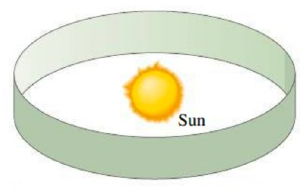
\includegraphics[scale=0.6]{figures/q4.PNG}
\end{figure}
\noindent
A science-fiction story describes an artificial ``planet'' in the form of a band completely encircling a sun, as in the figure. The inhabitants live on the interior surface (where it is always noon). Imagine that this sun is exactly like our own, that the distance to the band is the same as the Earth-Sun distance and that the ring rotates sufficiently quickly to produce an apparent gravity of $g$, as on Earth. What will be the period of revolution, i.e., this planet's year, in terms of the following quantities? 

\begin{itemize}
    \item $g$: Gravitational acceleration on the Earth
    \item $r$: Distance from the sun to the ring-planet
    \item $M$: Mass of the sun
    \item $G$: Universal gravitational constant
    \item Gravitational force between masses $M$ and $m$: $F=G\frac{Mm}{r^2}$
\end{itemize}
\end{document}
